%vim:foldmethod=marker
\documentclass{article}
\usepackage{natbib}
\usepackage{paper}
\usepackage{xcolor}
\usepackage{tikz}
\usepackage{xr}
\externaldocument{ordinal_outcomes_appendix}


% ----------------------------- Title & Author ------------------------------ %
\title{Causal Inference with Ordinal Outcomes: Flexible Estimation Framework Using Normalizing Flows}
\author{Chanhyuk Park}
\date{}
% --------------------------------------------------------------------------- %

\begin{document}
    \maketitle

\begin{abstract}
  Ordinal outcomes, such as Likert-type survey responses, are ubiquitous in political science, yet they pose distinctive challenges for causal inference. These outcomes are routinely analyzed by assigning numerical scores and applying linear models, despite longstanding concerns that ordinal responses do not identify treatment effects on an underlying cardinal scale without additional assumptions. Building on the classical identification result for ordinal outcomes and existing recommendations to report probability-based quantities, I develop a flexible likelihood-based framework for estimating distributional causal effects, including category-specific and cumulative treatment effects, which are invariant to admissible transformations of the latent scale. Existing approaches typically estimate these quantities using parametric ordered logit or ordered probit models, which rely on restrictive assumptions about the latent error distribution and index specification.
  This paper proposes a flexible likelihood-based estimation framework for ordinal causal inference using conditional normalizing flows. The proposed estimator flexibly learns the conditional distribution underlying observed ordinal responses without imposing a parametric latent error distribution, while preserving the likelihood-based structure familiar from classical ordered response models. The same framework accommodates both structured latent-index models and fully nonparametric conditional distribution estimators, allowing researchers to balance interpretability and modeling flexibility within a unified estimation procedure.
  Monte Carlo simulations show that the proposed estimator maintains low bias across a broad range of latent error distributions and nonlinear response mechanisms under which conventional ordered response models perform poorly. Replications of two published survey experiments demonstrate that flexible distributional estimation can materially alter substantive conclusions about experimental treatment effects.
\end{abstract}

\newpage
\section{Introduction}
\label{sec:introduction}

Causal inference has become a central organizing principle in political science. Experimental and quasi-experimental designs, including survey experiments, difference-in-differences, and regression discontinuity designs, are now standard empirical strategies for studying the effects of policies, institutions, and information. Survey experiments are particularly prominent because random assignment provides a transparent basis for causal identification. Between 2021 and 2024, roughly 20\% of articles published in the \textit{American Political Science Review}, \textit{American Journal of Political Science}, and \textit{Journal of Politics} employed a survey experiment as part of their empirical strategy.

Many of these studies investigate outcomes that are inherently latent, including support for redistribution \citep{Alt2017a, Magni2021a}, evaluations of political leaders \citep{Canes-Wrone2002a, Kriner2009a}, and foreign policy preferences \citep{Tomz2020a}. Although these concepts are commonly viewed as lying on an underlying continuous attitude scale, they are almost always observed through ordinal response categories such as Likert-type scales ranging from \textit{strongly disagree} to \textit{strongly agree}. Consequently, causal inference in political science routinely relies on outcomes that preserve the ordering of responses but not the distances between them.

Applied researchers typically analyze ordinal outcomes in one of three ways. The most common approach assigns numerical scores to response categories and estimates treatment effects using difference-in-means or ordinary least squares, implicitly treating ordinal responses as cardinal. Another common strategy collapses multiple categories into a binary outcome before estimation, sacrificing information about intermediate responses. A third approach fits ordered response models, such as ordered logit or ordered probit, which explicitly account for the ordinal nature of the data through a latent-variable representation. Each approach reflects a different set of assumptions about the relationship between the observed ordinal responses and the underlying latent attitude.

This paper begins from a classical observation in the ordinal response literature: latent treatment effects are identified only up to location and scale transformations of the underlying latent variable. Consequently, treatment effects defined through arbitrary numerical codings of ordinal responses generally require additional measurement assumptions linking the observed categories to a cardinal latent scale \citep{Schroder2017a, Bond2018a, Bloem2022a}. This observation motivates a focus on distributional causal quantities, such as category-specific and cumulative treatment effects, which are defined directly on the observed ordinal responses and do not rely on assumptions about the cardinal spacing between adjacent categories.

This perspective complements recent recommendations in political methodology to summarize ordinal treatment effects using predicted probabilities rather than latent coefficients \citep{Hanmer2013a}. Rather than revisiting how ordered response models should be interpreted, this paper asks how these probability-based causal quantities should be estimated when the assumptions underlying conventional ordered response models are difficult to justify. The methodological focus therefore shifts from interpreting latent coefficients to flexibly estimating the conditional ordinal response distribution. Existing semiparametric estimators relax some of these assumptions but remain difficult to apply with rich covariate structures or nonlinear response mechanisms that are common in modern survey research.

Estimating these distributional causal effects requires modeling the conditional distribution of ordinal responses. Ordered logit and ordered probit remain the workhorses of applied political science because they efficiently exploit the ordering of response categories, admit interpretable latent-variable representations, and often perform well when their assumptions are approximately satisfied. Their validity, however, depends on assumptions about the latent error distribution and index specification that may be difficult to justify in many survey experiments. Political attitudes are frequently polarized or clustered, producing multimodal latent distributions, while persuasive treatments often affect moderate respondents differently from strong supporters, generating nonlinear treatment-response relationships. In such settings, misspecification can distort estimated category probabilities and cumulative treatment effects, even when the experimental design itself identifies the causal effect. The practical challenge is therefore not causal identification, but flexible estimation of the conditional ordinal response distribution.

This paper develops a flexible likelihood-based framework for estimating causal effects with ordinal outcomes. The proposed estimator employs conditional normalizing flows to model the conditional response distribution without imposing a fixed parametric latent error distribution. Unlike existing semiparametric estimators, the framework remains computationally feasible with high-dimensional covariates while preserving exact likelihood-based inference. A single estimation procedure spans classical latent-index models, generalized latent-index specifications, and fully nonparametric conditional response distributions, allowing researchers to balance structural assumptions and modeling flexibility while targeting the same probability-based causal quantities.

I evaluate the proposed framework through Monte Carlo simulations designed to reflect empirically realistic survey settings, including polarized latent attitudes, nonlinear treatment-response relationships, and non-Gaussian latent error distributions. Across these settings, the proposed estimator maintains low bias while conventional ordered response models exhibit substantial distortions in estimated probability effects. I then revisit the survey experiments of \citet{Tomz2020a} and \citet{Mattingly2025a}, showing that flexible estimation of the ordinal response distribution can materially alter substantive conclusions regarding the magnitude and distribution of treatment effects.

The remainder of the paper proceeds as follows. Section~\ref{sec:causalordinal} formalizes causal inference with ordinal outcomes and motivates distributional causal estimands. Section~\ref{sec:estimation} reviews existing estimation approaches and introduces the proposed likelihood-based framework. Section~\ref{sec:simulation} evaluates finite-sample performance through Monte Carlo simulations. Section~\ref{sec:application} presents the empirical applications. Section~\ref{sec:conclusion} concludes.

\clearpage



\section{Causal Inference with Ordinal Outcomes}
\label{sec:causalordinal}

This section develops the conceptual framework underlying the remainder of the paper. I begin by describing ordinal survey responses as measurements of an underlying latent attitude using the classical threshold-crossing model. I then revisit a well-known identification result showing that latent treatment effects are identified only up to location and scale, and discuss its implications for causal inference with ordinal outcomes. To address this nonidentification, I define distributional causal estimands on the probability scale and prove their identification under standard causal assumptions. Finally, I use a toy example to demonstrate why traditional approaches that assign arbitrary numerical scores to ordinal categories can lead to severe inferential errors, including sign flips in the estimated treatment effect.

\subsection{Latent Outcomes, Ordinal Responses, and Causal Effects}
\label{subsec:setup}

% fig:latent {{{
\begin{figure}[ht]
\centering
\begin{tikzpicture}[x=1cm,y=2.0cm]
  % Draw x-axis
  \draw[->,thick] (-5,0)--(5.2,0) node[right] {$Y_i^*$};
  
  % Draw thresholds (2 thresholds for 3 categories)
  \draw[thick] (-2,-.15)--(-2,.15) node[below=20pt] {$\alpha_1$};
  \draw[thick] (2,-.15)--(2,.15) node[below=20pt] {$\alpha_2$};
  
  % Category labels at the top
  \node[above,font=\small] at (-3.3,-0.75) {Category 1};
  \node[above,font=\small] at (0,-0.75) {Category 2};
  \node[above,font=\small] at (3.3,-0.75) {Category 3};
  
  % Control curve (wider)
  \draw[thick, blue] plot[smooth] coordinates {
    (-4.50,0.04) (-3.86,0.09) (-3.21,0.19) (-2.57,0.34) (-1.93,0.53) (-1.29,0.73) (-0.64,0.88) (0.00,0.94) (0.64,0.88) (1.29,0.73) (1.93,0.53) (2.57,0.34) (3.21,0.19) (3.86,0.09) (4.50,0.04)
  };
  
  % Treatment curve (narrower, higher peak)
  \draw[thick,dashed, red] plot[smooth] coordinates {
    (-4.50,0.00) (-3.86,0.00) (-3.21,0.00) (-2.57,0.03) (-1.93,0.13) (-1.29,0.44) (-0.64,0.97) (0.00,1.40) (0.64,1.34) (1.29,0.84) (1.93,0.35) (2.57,0.10) (3.21,0.02) (3.86,0.00) (4.50,0.00)
  };
  
  % Text labels for curves
  \node[above, blue] at (-2.4,0.6) {Control};
  \node[above, red] at (2.4,0.9) {Treatment};
\end{tikzpicture}

\caption{Ordinal responses arise by partitioning an underlying latent attitude into ordered response categories. The observed data identify how treatment changes probabilities of falling into response categories, but not the absolute scale of the latent attitude.}
\label{fig:latent}
\end{figure}
% }}}

Many quantities of interest in political science, such as support for redistribution \citep{Alt2017a, Magni2021a}, immigration preferences \citep{Mayda2005a}, trust in institutions, and foreign policy attitudes \citep{Scheve2001r, Tomz2020a}, are naturally viewed as continuous latent constructs. Survey respondents, however, rarely report these attitudes on a continuous scale. Instead, researchers observe ordinal responses, such as Likert items ranging from \textit{strongly disagree} to \textit{strongly agree}, ordered approval categories, or frequency scales. Consequently, empirical analyses are conducted using outcomes that preserve the ordering of respondents’ attitudes but not the distances between adjacent response categories.

Following the classical ordered response framework, let $Y_i^\ast$ denote respondent $i$’s latent attitude and let $Y_i\in\{0,1,\ldots,J\}$ denote the observed ordinal response. The observed response is generated through a threshold-crossing mechanism,
\[
Y_i=j \quad\Longleftrightarrow\quad \alpha_{j-1}<Y_i^\ast\le\alpha_j,
\qquad j=0,\ldots,J,
\]
where
\[
-\infty=\alpha_{-1}<\alpha_0<\cdots<\alpha_J=\infty
\]
are unknown thresholds partitioning the latent scale. Figure~\ref{fig:latent} illustrates this measurement process. Throughout the paper, I assume respondents share a common reporting function (see Appendix~\ref{app:heterogeneous} for extensions allowing heterogeneous reporting thresholds across respondents).

The threshold-crossing representation serves as a measurement model that formalizes how ordinal responses preserve the ordering of underlying attitudes while discarding information about cardinal distances between adjacent categories. To describe causal effects, let $Y_i^\ast(d)$ denote the latent potential outcome under treatment level $d \in \{0,1\}$, and let $Y_i(d) = g\left(Y_i^\ast(d)\right)$ denote the corresponding observed ordinal potential outcome. Throughout, I adopt standard causal assumptions: SUTVA, conditional ignorability, and positivity \citep{Rubin1974a}.

This latent variable structure connects directly to the theory of signed causal diagrams and monotonic causal effects \citep{VanderWeele2010a, VanderWeele2012a}. When a treatment $D_i$ exerts a monotonic positive effect on the latent attitude $Y_i^\ast$, it implies that $Y_i^\ast(1) \ge Y_i^\ast(0)$ for all units. In terms of observed ordinal responses, this latent monotonic shift induces a relationship of \emph{first-order stochastic dominance} on the potential outcome distributions: $P(Y_i(1) \ge j) \ge P(Y_i(0) \ge j)$ for all categories $j$. 

However, because $Y_i^\ast$ is observed only through discrete categories, analyzing ordinal outcomes by assigning arbitrary numerical scores $c(0) < c(1) < \cdots < c(J)$ to calculate mean differences can lead to severe inferential errors. To see why cardinalization is fundamentally fragile, consider a simple toy example. Suppose an outcome has three ordered categories ($1 = \text{\textit{Disagree}}$, $2 = \text{\textit{Neutral}}$, $3 = \text{\textit{Agree}}$). A treatment alters the outcome distribution such that the category-specific probability differences between treatment and control, $P(Y_i(1)=j) - P(Y_i(0)=j)$, are:

\[
  \begin{aligned}
     P(Y_i(1)=1) - P(Y_i(0)=1) &= -0.15 \\
     P(Y_i(1)=2) - P(Y_i(0)=2) &= 0.25 \\
     P(Y_i(1)=3) - P(Y_i(0)=3)) &= -0.10 \\
  \end{aligned}
\]

In plain terms, the treatment shifts respondents away from the extreme categories by reducing \textit{Disagree} responses by 15 percentage points and \textit{Agree} responses by 10 percentage points, and concentrates mass in the moderate \textit{Neutral} category (an increase of 25 percentage points).

Now consider two strictly monotonic, equally valid numerical scoring choices:
\begin{itemize}
    \item \textbf{Coding A:} $c_A = (1, 2, 3)$, assuming equal spacing between categories.
    \item \textbf{Coding B:} $c_B = (1, 2, 6)$, assuming the gap between \textit{Neutral} and \textit{Agree} is four times larger than between \textit{Disagree} and \textit{Neutral}.
\end{itemize}

Calculating the mean treatment effect $\tau_c = \sum_{j=1}^J c(j)\Delta_j$ under both codings yields diametrically opposed conclusions:
\begin{align*}
  \tau_{c_A} &= 1 \cdot (-0.15) + 2 \cdot (0.25) + 3 \cdot (-0.10) = \mathbf{+0.05}, \\
  \tau_{c_B} &= 1 \cdot (-0.15) + 2 \cdot (0.25) + 6 \cdot (-0.10) = \mathbf{-0.25}.
\end{align*}

Under Coding A, a researcher concludes that the treatment increases average support ($+0.05$). Under Coding B, analyzing the \emph{exact same data} leads to the conclusion that treatment decreases support ($-0.25$). This sign flip is not a matter of sampling noise or small-sample bias, but a fundamental identification failure caused by imposing arbitrary cardinal spacing on ordinal data. This failure strongly motivates establishing formal identification results for ordinal causal inference \citep{Schroder2017a, Bond2018a}.

\subsection{Identification of Causal Effects from Ordinal Outcomes}
\label{subsec:identification}

The threshold-crossing framework provides a useful representation of ordinal outcomes, but it also reveals a fundamental limitation of what can be learned from ordinal data. A classical result in the ordered response literature is that latent-variable models are identified only up to location and scale \citep{Klein1997a, Schroder2017a}. Although this normalization is standard in econometrics and psychometrics, its implications for causal inference have received comparatively little attention in applied political science. In particular, survey experiments frequently interpret treatment effects estimated from numerically coded ordinal responses as effects on an underlying latent attitude without making explicit the measurement assumptions required for such an interpretation.

To formalize this point, suppose the latent outcome satisfies

\begin{equation}
  Y_i^\ast = h(X_i) + D_i^\top\tau + \varepsilon_i,
\label{eq:latent}
\end{equation}

where $h(X_i)$ denotes the systematic component of the latent outcome, $\tau$ is the treatment effect on the latent scale, and $\varepsilon_i$ has cumulative distribution function $F$. I sometimes use $m(X_{i}, D_{i})$ to denote the whole systematic linear structure $h(X_{i}) + D^{\top}_{i}\tau $ Combining this latent-index specification with the threshold-crossing measurement model implies

\[
\begin{aligned}
  P(Y_i=j\mid X_i,D_i) &= F\left( \alpha_j-h(X_i,\beta)-D_i^\top\tau \right) \\
   &= F\left( \alpha_{j-1}-h(X_i,\beta)-D_i^\top\tau \right). \\
\end{aligned}
\]

Now consider any constants $a\in\mathbb{R}$ and $c>0$, and define a transformed latent outcome

\[
\tilde Y_i^\ast = a+cY_i^\ast,
\]

together with transformed thresholds

\[
\tilde\alpha_j = a+c\alpha_j.
\]

Because both the latent outcome and the thresholds are transformed simultaneously, the probabilities of the observed ordinal responses remain unchanged.

\begin{theorem}[Location and Scale Nonidentification]
\label{theorem:locationscale}
Under the threshold-crossing latent-variable model, any positive affine transformation of the latent outcome and thresholds generates the same distribution of the observed ordinal responses. Consequently, treatment effects on the latent outcome are identified only up to location and scale.
\end{theorem}

Theorem~1 should not be interpreted as a failure of causal identification. Under the standard assumptions of SUTVA, conditional ignorability, and positivity, causal effects remain identified for any well-defined outcome. Rather, the theorem highlights a measurement problem. Ordinal responses preserve the ordering of latent attitudes but do not reveal the cardinal scale on which those attitudes are measured. Consequently, causal quantities defined on the latent scale require additional measurement assumptions beyond those needed for causal identification itself.

This distinction has immediate implications for empirical practice. Different analyses of ordinal outcomes target different causal quantities and therefore rely on different measurement assumptions. For example, assigning numerical scores to ordinal categories and estimating mean differences implicitly assumes that those scores provide a meaningful cardinal representation of the latent attitude. By contrast, causal quantities defined directly on the observed ordinal responses do not require assumptions about the cardinal spacing between adjacent categories. The next subsection formalizes these probability-based causal estimands and shows how they arise naturally from the observed ordinal response distribution.


\subsection{Distributional Causal Estimands}
\label{subsec:estimands}

The identification result in Theorem~1 does not imply that causal inference with ordinal outcomes is fundamentally limited. Rather, it suggests that inference should focus on causal quantities defined directly on the observed ordinal responses. Such quantities require no assumptions about the cardinal spacing of the latent attitude and therefore remain invariant to admissible transformations of the latent scale. This perspective is closely aligned with recommendations to report predicted probabilities rather than latent coefficients when interpreting ordinal response models \citep{Greene2010a, Hanmer2013a}. Here I formalize these quantities as causal estimands and show that they are identified under the standard assumptions of causal inference.

The fundamental object is the distribution of potential ordinal outcomes. Let

\[
\pi_j(d) = P\left( Y_i(d)=j \right),
\qquad j=0,\ldots,J,
\]

denote the probability that a randomly selected individual reports category $j$ under treatment level $d$.

\begin{theorem}
  \label{theorem:prob_id}
Under the standard assumptions of SUTVA, conditional ignorability, and positivity, these probabilities are identified by standardization,

\[
\pi_j(d) = \mathbb{E}_X\left[P\left( Y_i=j \mid D_i=d,X_i \right)\right],
\]

where the expectation is taken over the covariate distribution of the target population. In randomized experiments, this expression simplifies to the observed proportion of respondents falling into category $j$ within each treatment arm.
\end{theorem}

\begin{proposition}
  Based on Theorem~\ref{theorem:prob_id}, any causal quantity that is a functional of this distribution is also identified.
\end{proposition}

This proposition has an important practical implication. Once the conditional ordinal response distribution has been estimated, a wide range of causal quantities become available without fitting additional models. The primary statistical task is therefore estimation of the conditional response probabilities,

\[
P(Y_i=j\mid D_i,X_i),
\]

which serve as the building blocks for all distributional causal estimands considered in this paper.

The simplest causal quantity is the category-specific treatment effect,

\[
\Delta_j = \pi_j(1)-\pi_j(0),
\]

which measures how treatment changes the probability that a respondent selects category $j$. For example, in a survey experiment on support for military intervention, $\Delta_{\text{Strongly Agree}}$ measures the change in the proportion of respondents expressing the strongest level of support.

In many political science applications, however, interest centers on whether respondents exceed a substantively meaningful threshold rather than on a single response category. This motivates cumulative treatment effects,

\[
\Delta_{\ge j} = P\left( Y_i(1)\ge j \right) = P\left( Y_i(0)\ge j \right),
\]

which quantify changes in the probability of responding at or above category $j$. For example, a researcher may wish to estimate whether an informational treatment increases the probability that respondents express at least moderate support for a policy. Unlike dichotomizing the outcome before estimation, cumulative treatment effects can be calculated for every threshold after estimating the ordinal response distribution, allowing the full information contained in the ordinal responses to be retained.

These estimands also clarify the relationship between the proposed framework and existing empirical practice. Assigning numerical scores to ordinal categories estimates

\[
\mathbb{E} = \left[ s(Y_i(1))-s(Y_i(0)) \right],
\]

where $s(\cdot)$ denotes the chosen scoring rule. This quantity is well defined for a fixed coding rule but generally does not identify a treatment effect on the underlying latent attitude. Similarly, dichotomizing an ordinal outcome estimates one cumulative treatment effect corresponding to a single threshold while discarding information about the remaining response categories. Estimating the full ordinal response distribution instead makes both category-specific and cumulative treatment effects available simultaneously, allowing researchers to select the quantity most appropriate for their substantive question after estimation rather than before it.

The discussion above highlights an important feature of distributional causal inference. Rather than targeting a single summary measure, the primary object of interest is the conditional distribution of ordinal responses,
\[
P(Y_i=j\mid D_i,X_i),
\]
from which a wide range of causal quantities can be obtained. Category-specific treatment effects and cumulative treatment effects are the primary estimands considered in this paper because they are directly interpretable and commonly reported in applied political science. More generally, however, any functional of the estimated response distributions may be calculated after estimation, including global measures of distributional change such as the one-dimensional Wasserstein (earth mover's) distance. Consequently, the statistical problem addressed in the remainder of this paper is estimation of the conditional ordinal response distribution rather than any single causal summary.

\section{Flexible Estimation of Ordinal Response Distributions}
\label{sec:estimation}

Section~\ref{sec:causalordinal} established that the causal quantities of interest are functionals of the conditional ordinal response distribution,
\[
P(Y_i=j\mid D_i,X_i).
\]
The remaining statistical problem is therefore estimation of this distribution. This section first reviews existing estimation approaches and their underlying assumptions before introducing a flexible likelihood-based framework that generalizes classical ordered response models while preserving their probabilistic interpretation.

\subsection{Existing Estimation Approaches}
\label{subsec:existing}

The dominant approach to modeling ordinal outcomes in political science is the ordered response model, most commonly ordered logit or ordered probit. These models combine the latent-index representation in Equation~\eqref{eq:latent} with the threshold-crossing measurement model introduced in Section~\ref{subsec:setup}. By imposing a strict parametric structure on both the systematic component (a linear index) and the latent error distribution (normal or logistic), these models are highly efficient. Political methodologists have long recognized the limitations of rigid, symmetric error distributions, prompting early parametric generalizations such as the \textit{scobit} (skewed logit) model \citep{Nagler1994a}, which introduces an additional parameter to accommodate asymmetric latent tails. Yet, while scobit relaxes symmetry, it remains constrained within a fixed parametric family. In small samples (e.g., $N < 500$) or when prior theoretical knowledge strongly dictates a symmetric, unimodal response process, ordered probit and logit remain excellent choices. However, when attitudes are polarized (multimodal), heteroskedastic, or subject to ceiling and floor effects, these rigid parametric assumptions induce severe bias, distorting the estimated category probabilities that form the basis of substantive interpretation.

On the opposite end of the methodological spectrum, because category-specific treatment effects are nonparametrically identified, one could discard models entirely and rely on a fully nonparametric empirical frequency estimator. This approach computes conditional category probabilities directly from observed sample proportions in each treatment-covariate cell. While asymptotically unbiased and consistent, this robust nonparametric property comes at a severe cost in finite samples. In the sample sizes typical of empirical survey experiments, the fully nonparametric estimator suffers from the curse of dimensionality. It cannot easily incorporate continuous baseline covariates, and it is highly vulnerable to sparse-data issues, possibly resulting in enormous estimation variance. 

This creates a fundamental bias-variance tradeoff: standard parametric models have low variance but high bias under misspecification, while fully nonparametric estimators are unbiased but suffer from crippling finite-sample variance. 
The most effective estimator for modern survey experiments should therefore occupy a middle ground that exploits structural information from the data without imposing restrictive parametric distributional assumptions. This logic mirrors the classical relationship between linear regression and raw difference-in-means estimators: while a simple difference-in-means is fully nonparametric, researchers routinely use OLS to efficiently pool information across covariates and reduce finite-sample variance. Applying this principle to ordinal outcomes, a structured "middle ground" estimator would retain the parametric linear index $h(X_i) + D_i^\top\tau$ to leverage covariate-driven precision gains and borrow strength across adjacent categories, while completely relaxing the parametric assumption on the latent error distribution $F(\cdot)$. 

While several flexible machine learning approaches exist, they generally struggle to effectively occupy this middle ground for ordinal data. For instance, tree-based methods like Causal Forests \citep{Breiman2001a} are excellent for high-dimensional covariate adjustment, but they typically handle ordinal outcomes poorly. They either treat ordinal responses as continuous (imposing the arbitrary cardinal scores critiqued in Section~\ref{subsec:setup}) or require estimating separate binary forests for each threshold $P(Y \le j)$. The latter approach ignores the joint ordinal structure and frequently produces "crossing" thresholds (e.g., predicting $P(Y_i \le 2) < P(Y_i \le 1)$), resulting in mathematically impossible negative category probabilities. Alternatively, Bayesian nonparametric models \citep{Zhou2019a} can successfully estimate flexible error distributions without crossing thresholds, but they rely on computationally intensive Markov Chain Monte Carlo (MCMC) sampling. Consequently, they scale poorly to large datasets and high-dimensional covariate spaces. 

The preceding discussion suggests that the objective is not simply to throw off-the-shelf machine learning at ordinal data, nor to stubbornly cling to the normal distribution. Rather, the goal is to estimate the conditional ordinal response distribution while strictly preserving the probabilistic threshold-crossing structure that makes classical models coherent, and to do so using a scalable, likelihood-based procedure. The next subsection introduces a Conditional Normalizing Flow framework designed specifically to meet these criteria.

\subsection{A Flexible Likelihood-Based Framework}
\label{subsec:framework}

The preceding discussion suggests that the objective is not simply to replace the normal or logistic error distribution with a more flexible alternative. Rather, the goal is to estimate the conditional ordinal response distribution while preserving the probabilistic structure that makes ordered response models attractive. 

The proposed Conditional Normalizing Flow (CNF) framework bridges this gap, positioning itself as an optimal compromise on the efficiency-robustness frontier. Like standard parametric models, the CNF retains high statistical efficiency and finite-sample stability: it can explicitly models the systematic component $m(X_i, D_i)$ to leverage covariate-driven precision gains, and utilizes the ordered threshold-crossing structure to borrow strength across adjacent categories, mitigating sparse-data and zero-cell issues. At the same time, like the empirical frequency estimator, the CNF remains robust to distributional misspecification by learning the shape of the latent error distribution $F(\cdot)$ directly from the data. The resulting estimator thus combines the covariate-adjustment and smoothing advantages of parametric regression with the distributional flexibility of nonparametric frequency estimators.

Under this unified framework, the latent outcome representation in Equation~\eqref{eq:latent} is preserved, but we generalize how its individual components are modeled. Recall that the latent outcome consists of two parts: the systematic component $m(X_i, D_i)$ and the latent error distribution $F(\cdot)$. Existing estimators correspond to restrictive choices of these two components. Ordered logit and ordered probit specify both parts parametrically, whereas semiparametric estimators typically relax only the latent error distribution.

The proposed framework allows flexibility in either or both components while retaining a common likelihood-based estimation procedure. When substantive theory suggests that treatment and covariates operate through a common latent index, the systematic component may be specified parametrically while the latent error distribution is estimated flexibly. This specification may be viewed as a semiparametric generalization of ordered response models. Alternatively, when the functional relationship between covariates and the latent outcome is itself uncertain, the systematic component may also be estimated nonparametrically. In this way, the same estimation framework spans classical latent-index models, semiparametric ordered response models, and fully flexible conditional distribution estimators without requiring different inferential procedures.

The framework is implemented using conditional normalizing flows to model unknown probability distributions. Unlike kernel-based semiparametric estimators, conditional normalizing flows scale naturally to high-dimensional conditioning variables while retaining exact likelihood evaluation. Consequently, they preserve the familiar inferential machinery of ordered response models, including maximum-likelihood estimation, likelihood-based model comparison, and probabilistic calibration, while substantially relaxing distributional assumptions.

A particularly attractive feature of ordinal response models is that the latent error is scalar. Combined with monotone normalizing flows, this permits exact evaluation of both the latent density and its cumulative distribution function. Consequently, the threshold-crossing likelihood can be evaluated exactly without numerical integration, allowing the proposed estimator to remain computationally tractable while flexibly modeling the latent error distribution.

In addition, the CNF framework also bridges the gap between structural choice models and modern semiparametric causal inference. Because probability-based effects are nonparametrically identified, recent econometric literature has increasingly relied on Double Machine Learning (DML) and Efficient Influence Functions (EIF) to isolate distributional and ordinal treatment effects \citep{Chernozhukov2013b}. A major practical challenge in applying DML to ordinal outcomes, however, is that estimating the nuisance parameters $P(Y_i \le j \mid X_i, D_i)$ independently for each threshold often leads to crossing predictions in finite samples. For example, predicting that $P(Y_i \le 2) < P(Y_i \le 1)$, yielding mathematically impossible negative category probabilities.

While the primary objective of this paper is to directly estimate the structural shape of the conditional ordinal response distribution, the CNF framework provides a natural solution for researchers who wish to pursue formal semiparametric efficiency. By jointly modeling the entire distribution through a single, strictly monotonic latent transformation, the CNF guarantees that the estimated cumulative probabilities never cross. Consequently, the proposed flow-based estimator can serve as a highly efficient, structure-preserving nuisance estimator that can be plugged directly into existing EIF/AIPW pipelines for doubly robust estimation.


\subsection{Modeling the Latent Error Distribution with Normalizing Flows}
\label{subsec:flow}

% fig:nf_error {{{
\begin{figure}[hb!]
\vspace{1cm}
\centering
\begin{tikzpicture}[>=stealth,scale=1]

% --------------------------------------------------
% Left panel: base distribution
% --------------------------------------------------
\begin{scope}[shift={(-4.6,0)}]
    \draw[thick] (-2.1,0) rectangle (2.5,3.0);
    \draw[->] (-1.75,0.25) -- (1.75,0.25) node[right] {\small $z$};
    \draw[->] (-1.75,0.25) -- (-1.75,2.35) node[above right] {\small $p_Z(z)$};

    \draw[thick]
    plot[smooth]
    coordinates{
        (-1.6,0.28)
        (-1.2,0.35)
        (-0.8,0.75)
        (-0.4,1.65)
        (0,2.25)
        (0.4,1.65)
        (0.8,0.75)
        (1.2,0.35)
        (1.6,0.28)
    };

    \node at (0,-0.35) {\small Base distribution};
    \node at (0,-0.75) {\small $z\sim N(0,1)$};
\end{scope}

% --------------------------------------------------
% Middle: conditional normalizing flow
% --------------------------------------------------
\node[draw, rounded corners, align=center, minimum width=2.8cm, minimum height=1.1cm]
    (flow) at (0,1.25)
    {\small Conditional\\[-0.1em]\small normalizing flow\\[-0.1em]\small $T_\phi(\cdot\mid D_i,X_i)$};

\draw[->,thick] (-2 ,1.55) -- (-1.4, 1.45);
\draw[->,thick] (1.4, 1.45) -- (2.25,1.55);

\node[align=center] at (0,2.55)
    {\small Generative direction:\\[-0.1em]
     \small $\varepsilon_i=T_\phi(z_i\mid D_i,X_i)$};

\node[align=center] at (0,-0.55)
    {\small Normalizing direction:\\[-0.1em]
     \small $z_i=T_\phi^{-1}(\varepsilon_i\mid D_i,X_i)$};

\draw[<-,thick,dashed] (-2,0.85) -- (-1.4, 0.95);
\draw[<-,thick,dashed] (1.4, 0.95) -- (2.25,0.85);

% --------------------------------------------------
% Right panel: flexible latent error distribution
% --------------------------------------------------
\begin{scope}[shift={(4.6,0)}]
    \draw[thick] (-2.1,0) rectangle (2.5,3.0);
    \draw[->] (-1.75,0.25) -- (1.75,0.25) node[right] {\small $\varepsilon$};
    \draw[->] (-1.75,0.25) -- (-1.75,2.35) node[above right] {\small $f_\varepsilon(\varepsilon\mid D,X)$};

    \draw[thick]
    plot[smooth]
    coordinates{
        (-1.7,0.28)
        (-1.25,0.35)
        (-0.9,0.60)
        (-0.55,0.85)
        (-0.2,0.65)
        (0.15,0.45)
        (0.45,0.75)
        (0.75,1.65)
        (1.0,2.05)
        (1.25,1.20)
        (1.55,0.35)
        (1.8,0.28)
    };

    \node at (0,-0.35) {\small Flexible latent error};
    \node at (0,-0.75) {\small distribution};
\end{scope}

% --------------------------------------------------
% Bottom: ordered response connection
% --------------------------------------------------
\node[align=center] at (0,-1.75)
{\small Combined with the latent index and thresholds, the estimated error distribution implies\\[-0.1em]
 \small conditional ordinal probabilities $P(Y_i=j\mid D_i,X_i)$.};

\end{tikzpicture}
\caption{Normalizing Flows}
\label{fig:nf_error}
\begin{flushleft}
  {\footnotesize
A conditional normalizing flow transforms a simple base distribution into a flexible latent error distribution. In the proposed ordered-response framework, this replaces the fixed normal or logistic error assumption while retaining likelihood-based estimation.}
\end{flushleft}
\end{figure}
% }}}

Normalizing flows provide a natural framework for flexible density estimation. Originally introduced by \citet{Rezende2016a}, normalizing flows represent an unknown probability distribution through a sequence of invertible transformations of a simple base distribution. Because each transformation is strictly invertible, probability densities remain analytically tractable through the change-of-variables formula, allowing estimation to proceed directly by maximum likelihood \citep{Kobyzev2021a, Papamakarios2021a}.

Figure~\ref{fig:nf_error} illustrates the basic mechanism. Let $z_i\sim p_Z(z)$ denote a simple base distribution, taken throughout this paper to be the standard normal distribution. A conditional normalizing flow transforms this base distribution into the latent error distribution through an invertible mapping,
\[
\varepsilon_i = T_\phi(z_i\mid D_i,X_i),
\]
where the transformation is parameterized by $\phi$ and conditioned on the treatment and covariates. The same transformation may be inverted, $z_i = T_\phi^{-1}(\varepsilon_i\mid D_i,X_i)$, allowing observations to be mapped back to the base distribution. This invertibility enables exact likelihood evaluation through the standard change-of-variables formula:
\[
f_\varepsilon(\varepsilon_i\mid D_i,X_i) = p_Z(z_i)
\left|
\det \frac{\partial T_\phi^{-1}(\varepsilon_i\mid D_i,X_i)} {\partial\varepsilon_i}
\right|.
\]

Unlike kernel density estimators or generic deep neural networks, the transformation $T_\phi(\cdot)$ must guarantee strict monotonicity. We construct $T_\phi(\cdot)$ using monotonic rational-quadratic splines (RQS) \citep{Durkan2019a}. Intuitively, an RQS divides the continuous latent space into a set of $K$ distinct bins (or knots). Within each bin, it fits a smooth, strictly monotonic rational-quadratic polynomial. The parameters governing these bins (their widths, heights, and boundary derivatives) are outputted dynamically \footnote{The range of these hyperparameters can be set to further regulate the transformation} by a conditioning neural network based on $D_i$ and $X_i$. For our empirical implementations, we typically employ $K=8$ bins and a lightweight conditioner network (e.g., two hidden layers of 32 units). Because the RQS construction is piecewise analytical and one-dimensional, it provides extreme flexibility while permitting exact closed-form evaluation of both the inverse transformation and the implied cumulative distribution function (CDF). This crucial feature avoids the computationally expensive and unstable numerical integration required by other flexible ordered response estimators.

\subsection{Identification of the Latent Error Distribution}
\label{error_identification}
A fundamental theoretical question when relaxing the parametric error assumption is whether the observed ordinal data actually contain sufficient information to identify the shape of the unknown latent error distribution $F$. Following classical identification results for semiparametric index models \citep{Manski1988a, Klein1993a, Klein2002a}, the latent error distribution is nonparametrically identified provided the systematic index $m(X_i, D_i) = h(X_i) + D_i^\top\tau$ is sufficiently quasi-continuous. 

Specifically, identification requires at least one continuous covariate in $X_i$ with a non-zero coefficient (often termed a \textit{special regressor}) and sufficiently large support. Because the index acts as a shifting location parameter, continuous variation in $m(X_i, D_i)$ effectively sweeps the fixed measurement thresholds $\alpha_j$ across the support of $\varepsilon_i$. The observed threshold probabilities, 
\[
P(Y_i \le j \mid X_i, D_i) = F(\alpha_j - m(X_i, D_i)),
\]
thus continuously trace out the entire cumulative distribution function of the error term. This quasi-continuous variation ensures that the normalizing flow has a unique, identifiable distributional target to learn from the data, establishing the theoretical validity of our flexible estimator. Appendix~\ref{app:estimation} provides the formal statement of these regularity conditions and the resulting consistency theorem.

Ultimately, the conditional flow is used solely to model the latent error distribution $F$. As outlined in Section~\ref{subsec:framework}, this error distribution is then paired with either a parametric linear index (the \textit{Structured Flow}) or a fully nonparametric systematic component (the \textit{Model-Free Flow}). Both specifications share the same likelihood and estimation procedure, utilizing the exact CDF evaluated by the RQS flow.

\subsection{Likelihood-Based Estimation and Causal Estimands}
\label{subsec:likelihood}

The latent-index representation, together with the threshold-crossing measurement model introduced in Section~\ref{subsec:setup}, implies that the probability of observing response category $j$ is
\begin{align*}
P(Y_i=j\mid D_i,X_i) &= P\left( \alpha_{j-1} < Y_i^\ast \le \alpha_j \mid D_i,X_i \right) \\
&= F_\phi \left( \alpha_j - m(X_i, D_i) \mid D_i,X_i \right)
- F_\phi \left( \alpha_{j-1} - m(X_i, D_i) \mid D_i,X_i \right),
\end{align*}
where $m(X_i, D_i)$ is the systematic component (e.g., $h(X_i) + D_i^\top\tau$ in the \textit{Structured Flow}) and $F_\phi(\cdot)$ denotes the conditional cumulative distribution function implied by the RQS normalizing flow with parameters of $\phi$. This expression structurally mirrors ordered logit and ordered probit, differing only in that the latent error distribution $F_\phi$ is estimated directly from the data rather than assumed \textit{a priori}. 

Assuming independent observations, the log-likelihood for the observed ordinal responses is
\[
\ell(\Theta) = \sum_{i=1}^{n} \sum_{j=0}^{J} 1(Y_i=j) \log P(Y_i=j\mid D_i,X_i),
\]
where $\Theta$ collects all unknown parameters of the latent outcome model (parameters for $h(\cdot)$ and $\tau$), the conditional normalizing flow network ($\phi$), and the reporting thresholds ($\alpha$). These parameters, as denote by Theorem~\ref{theorem:locationscale}, only identified up to location and scale, unlike the distributional effect such as category-specific effects. 

The parameters are estimated by maximizing the likelihood using a combination of stochastic gradient-based Adam optimizer, and a quasi-Newton method. Because the one-dimensional RQS flow admits exact, closed-form evaluation of the cumulative distribution function, the resulting objective remains a genuine, exact log-likelihood rather than a numerical approximation or a surrogate prediction loss. Consequently, estimation retains the highly desirable features of classical ordered response models including likelihood-based estimation. Furthermore, because estimation proceeds by maximum likelihood over smooth, finite-dimensional spline parameters, standard asymptotic normality holds. This ensures the theoretical validity of the nonparametric bootstrap for post-estimation uncertainty quantification, a property that often fails for other nonparametric machine learning estimators like standard random forests \citep[see Appendix~\ref{app:estimation} for formal regularity conditions]{Bickel1981a}.

Once the model is fitted, it directly yields the strictly monotonic, non-crossing conditional probabilities $\widehat{P}(Y_i \le j \mid D_i, X_i)$ and $\widehat{P}(Y_i=j \mid D_i, X_i)$. These conditional probabilities serve as the fundamental building blocks for estimating distributional causal effects. Researchers can utilize these probabilities in two primary ways depending on their empirical design.

For randomized survey experiments, causal quantities are obtained by direct regression standardization, corresponding to the plug-in estimator of the g-formula \citep{Robins1986a}. For example, the estimated category-specific treatment effect is:

\[
\widehat{\Delta}_j = 
\frac{1}{n}
\sum_{i=1}^{n} \left[ \widehat{P}(Y_i=j\mid D_i=1,X_i) - \widehat{P}(Y_i=j\mid D_i=0,X_i) \right].
\]
Cumulative treatment effects are computed analogously:
\[
\widehat{\Delta}_{\ge j} = 
\frac{1}{n} \sum_{i=1}^{n} \left[ \widehat{P}(Y_i\ge j\mid D_i=1,X_i) - \widehat{P}(Y_i\ge j\mid D_i=0,X_i) \right].
\]

Alternatively, in observational settings with high-dimensional confounding, simple plug-in estimators may suffer from regularization bias. In such cases, the CNF's predicted probabilities can serve as first-stage nuisance estimators within a Double Machine Learning \citep[DML]{Chernozhukov2024a} or Targeted Maximum Likelihood Estimation \citep[TMLE]{Laan2006a} framework. By plugging the flow's conditional probabilities into the Augmented Inverse Probability Weighting \citep[AIPW]{Robins1994a} Efficient Influence Function (EIF), researchers can obtain doubly robust, root-$n$ consistent estimates of the causal estimands \citep{Chernozhukov2013b}. Crucially, because the CNF jointly models the distribution and strictly respects the ordinal thresholds, it completely eliminates the crossing probability errors that plague standard DML applications to ordinal outcomes. 

In sum, the proposed likelihood-based framework separates the task of statistical estimation from causal interpretation. The model is fitted once to learn the structural shape of the conditional response distribution, and substantive quantities of interest are subsequently obtained as mathematically coherent post-estimation functionals such as difference in probabilities in case of category-specific effects.

\clearpage

\section{Monte Carlo Simulation}
\label{sec:simulation}

\subsection{Simulation Design}
\label{subsec:sim_design}

Each simulation begins by generating a synthetic population of one million observations from the latent-index model in Equation~\eqref{eq:latent}. The latent outcome is converted into an observed ordinal response through the threshold-crossing measurement model introduced in Section~\ref{subsec:setup}, with common reporting thresholds fixed across treatment conditions. Because the population is sufficiently large, the true category-specific and cumulative treatment effects can be computed with negligible Monte Carlo error before sampling begins. Consequently, all reported estimation error reflects true finite-sample performance rather than uncertainty in the reference values.

Treatment assignment is completely randomized, ensuring that the identification assumptions developed in Section~\ref{sec:causalordinal} hold by construction. For each data-generating process, I draw 100 independent random samples of sizes $n\in\{500,1000,2000\}$ from the population. Each sampled dataset is analyzed independently, and performance measures are aggregated across Monte Carlo replications.

The simulation considers six data-generating processes designed to isolate different departures from the assumptions underlying classical ordered response models. Two benchmark settings generate latent errors from the normal and logistic distributions, under which ordered probit and ordered logit are correctly specified, respectively. The remaining settings introduce skewed latent errors, polarized (multimodal) latent attitudes, heteroskedastic latent errors, and nonlinear latent response functions. Together, these scenarios represent empirical features frequently encountered in survey experiments, allowing the consequences of different modeling assumptions to be examined separately.

Five estimators are compared, representing different points on the bias-variance tradeoff spectrum.
Empirical Distribution Estimator is a fully nonparametric approach that estimates category probabilities directly from observed treatment-arm frequencies. While asymptotically unbiased, it cannot easily incorporate covariates and suffers from high variance in finite samples.
Ordered Probit and Ordered Logit are fully parametric models that pool information efficiently but risk severe bias under misspecification.
Structured Flow is the proposed middle ground estimator that retains the linear latent-index model to borrow strength across covariates, while estimating the latent error distribution flexibly.
Model-Free Flow is a fully flexible specification that estimates not only the shape of the latent error distribution, but also the systematic component, $m(X_{i}, D_{i})$.

Performance is evaluated using bias, absolute bias, and root mean squared error (RMSE) for the distributional causal effects introduced in Section~\ref{subsec:estimands}. Because all estimators target the exact same causal estimands under identical identification assumptions, differences in performance reflect only the statistical consequences of the modeling choices.

\subsection{Simulation Results}
\label{subsec:sim_results}

\begin{figure}
  \begin{center}
  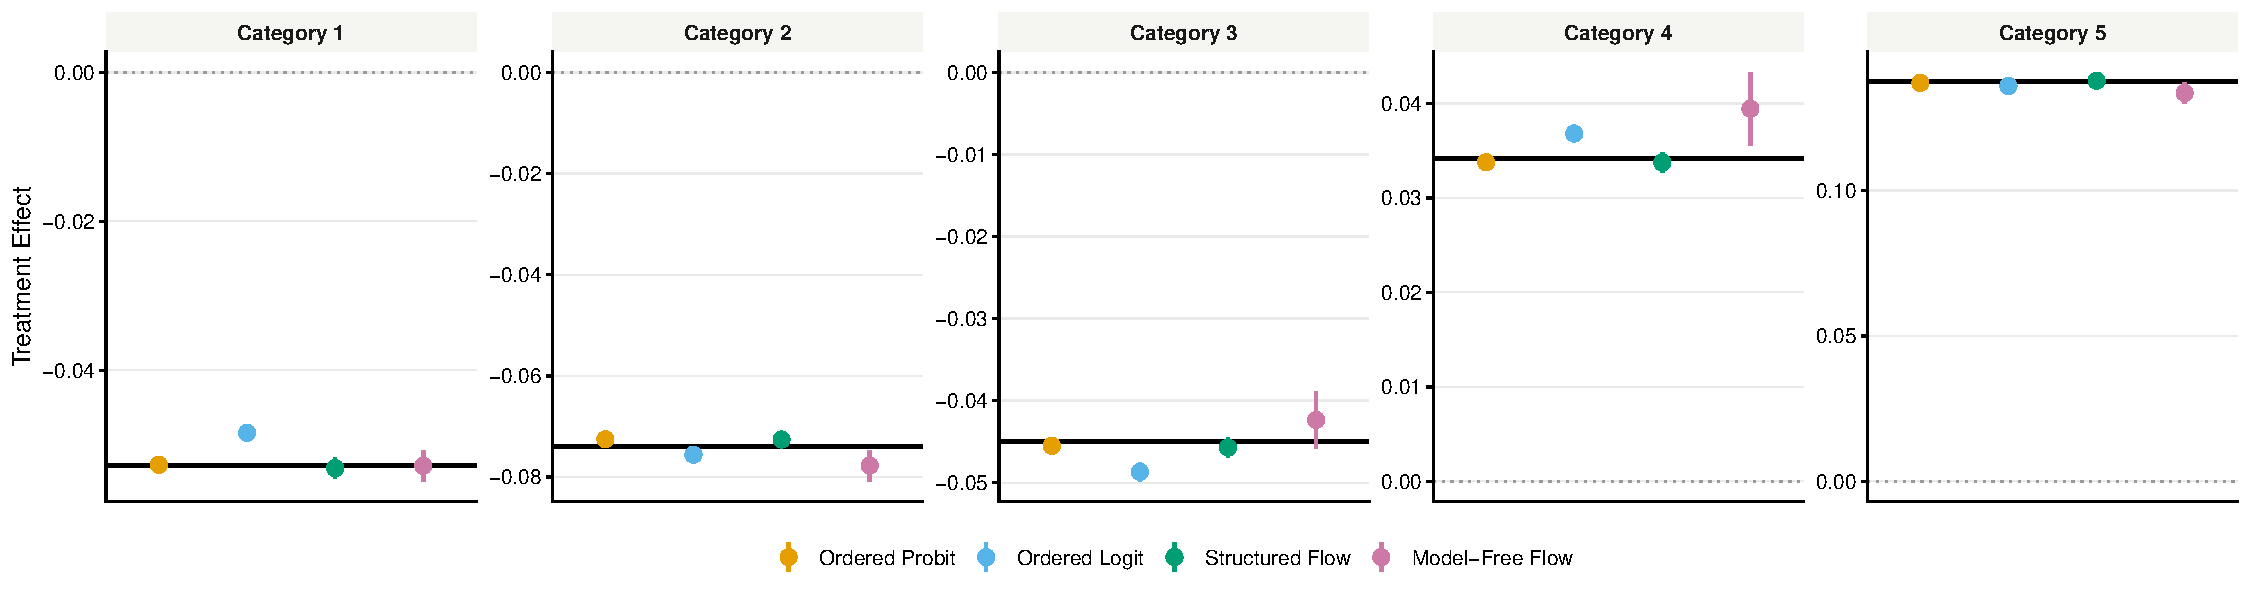
\includegraphics[width=0.95\textwidth]{../figures/fig_app_normal_linear_N2000.pdf}
  \end{center}
  \caption{Single Index Model with Normal Error}\label{fig:baseline}
  \vspace{0.5em}
  \footnotesize
  \begin{flushleft}
  \textit{Note:} This figure reports the estimated category-specific treatment effects with the corresponding population quantities when $n = 2000$. Points denote Monte Carlo averages across 100 replications, error bars indicate 95\% Monte Carlo confidence intervals, and the horizontal line marks the true population treatment effect.
  \end{flushleft}
\end{figure}

\begin{figure}
  \begin{center}
  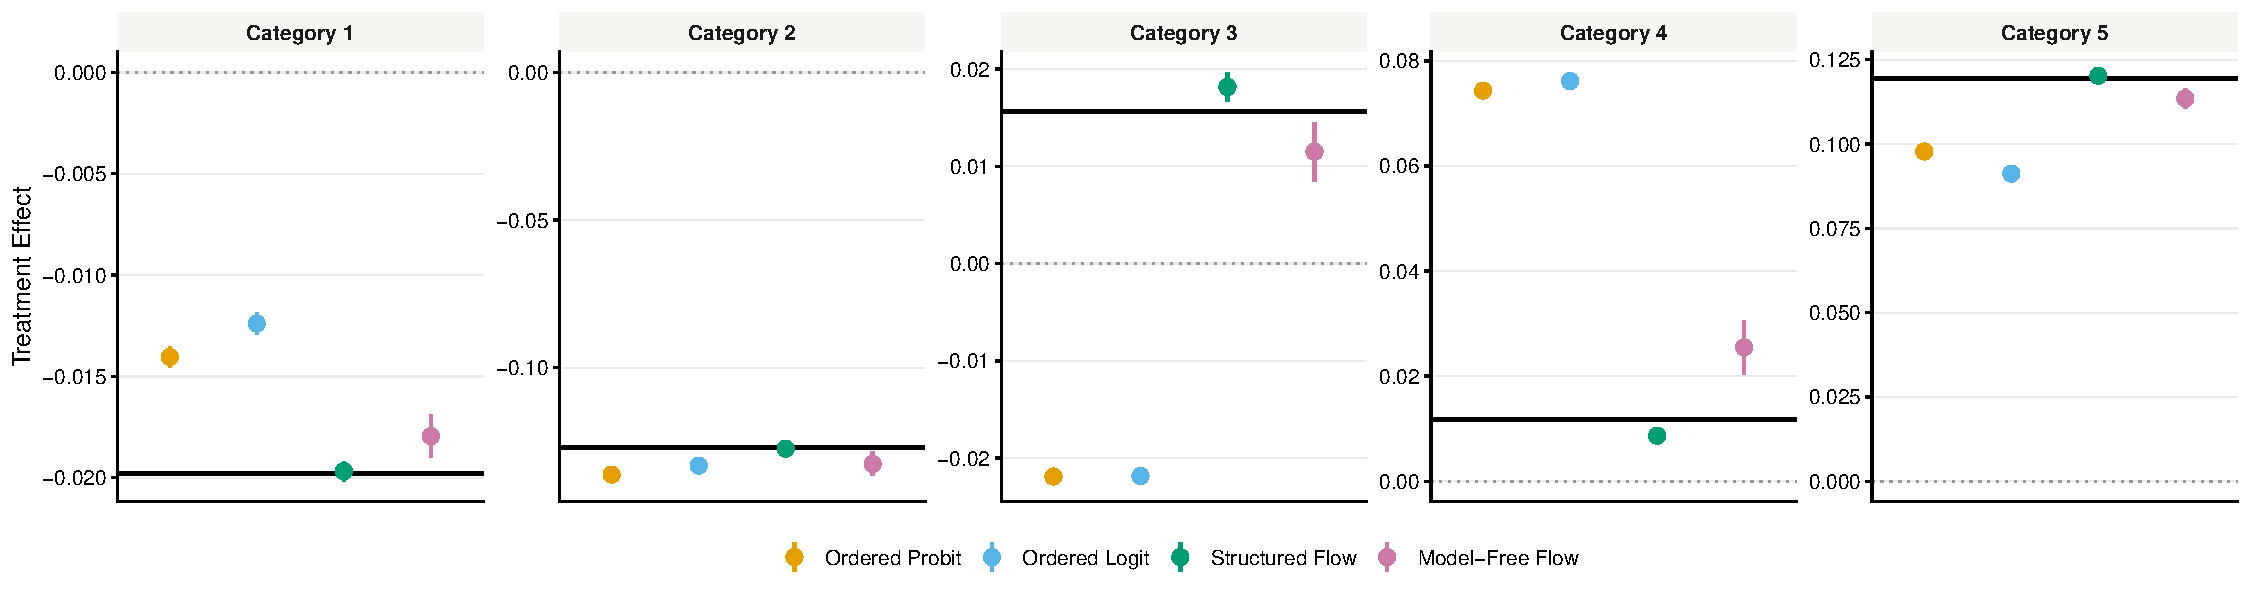
\includegraphics[width=0.95\textwidth]{../figures/fig_polarized_mixture_N2000.pdf}
  \end{center}
  \caption{Single Index Model with Bimodal Error}\label{fig:polarized}
  \vspace{0.5em}
  \footnotesize
  \begin{flushleft}
  \textit{Note:} This figure reports the estimated category-specific treatment effects with the corresponding population quantities when $n = 2000$. Points denote Monte Carlo averages across 100 replications, error bars indicate 95\% Monte Carlo confidence intervals, and the horizontal line marks the true population treatment effect.
  \end{flushleft}
\end{figure}

\begin{figure}
  \begin{center}
  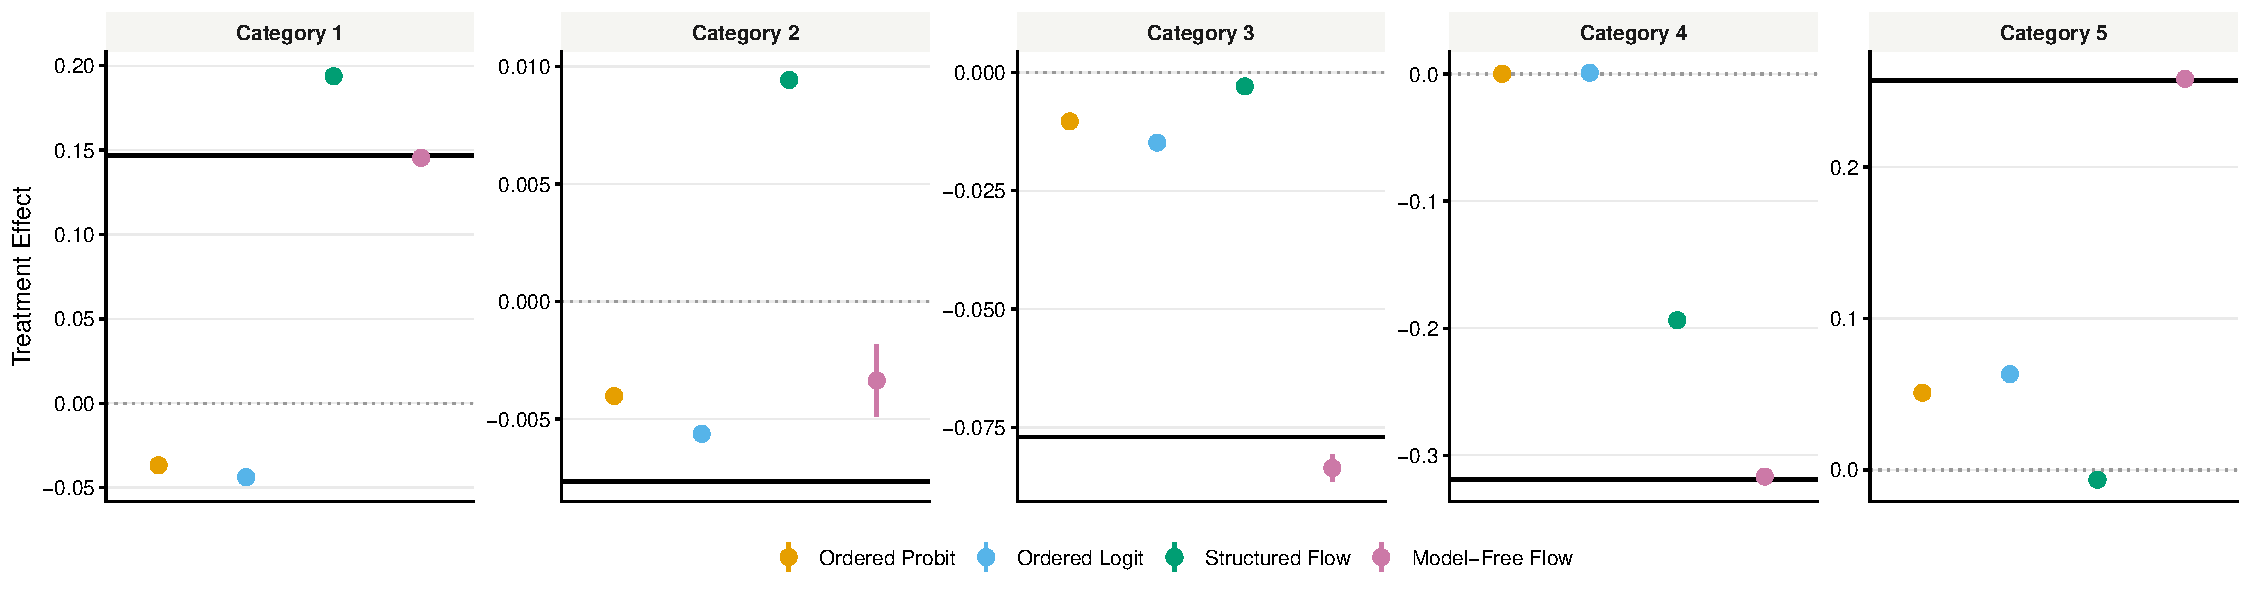
\includegraphics[width=0.95\textwidth]{../figures/fig_heteroskedastic_N2000.pdf}
  \end{center}
  \caption{Single Index Model with heteroskedastic Error}\label{fig:heteroskedastic}
  \vspace{0.5em}
  \footnotesize
  \begin{flushleft}
  \textit{Note:} This figure reports the estimated category-specific treatment effects with the corresponding population quantities when $n = 2000$. Points denote Monte Carlo averages across 100 replications, error bars indicate 95\% Monte Carlo confidence intervals, and the horizontal line marks the true population treatment effect.
  \end{flushleft}
\end{figure}

\begin{figure}
  \begin{center}
  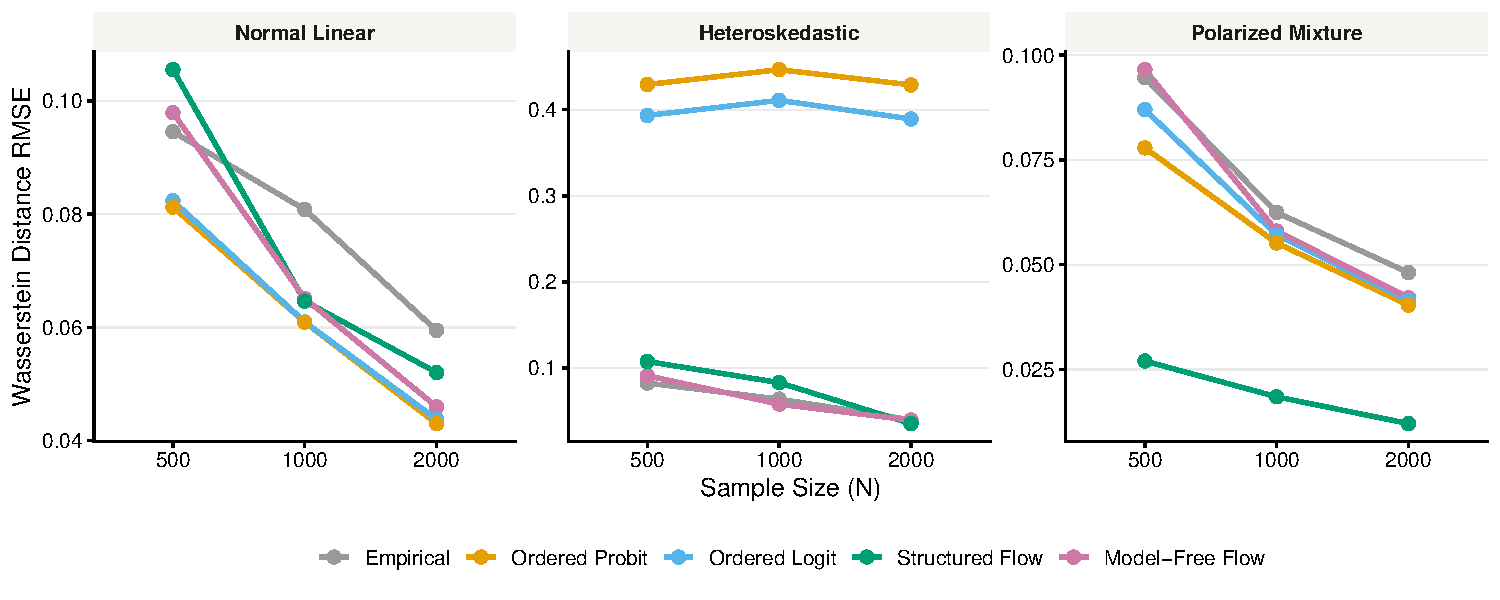
\includegraphics[width=0.95\textwidth]{../figures/fig_wasserstein_convergence.pdf}
  \end{center}
  \caption{Asymptotic Convergence (RMSE) in Wasserstein Distance}\label{fig:wasserstein}
  \vspace{0.5em}
  \footnotesize
  \begin{flushleft}
  \textit{Note:} This figure reports recovery of the entire conditional response distribution through the RMSE of the Wasserstein distance between the estimated and true distributions.
  \end{flushleft}
\end{figure}

The benchmark simulation in Figure~\ref{fig:baseline} provides an important validation of the bias-variance tradeoff. Under normally distributed latent errors, ordered probit is perfectly specified and statistically efficient. The raw empirical estimator is unbiased but exhibits noticeably wider confidence intervals. Crucially, the structured flow estimator performs comparably to ordered probit despite relaxing the parametric assumption on the latent error distribution. This indicates that flexibly modeling the error term incurs virtually no efficiency loss when the conventional model happens to be correct.

The advantages of the structured flow become apparent once the latent response mechanism departs from classical assumptions. Figure~\ref{fig:polarized} demonstrates that under a polarized (bimodal) mixture distribution, ordered logit and ordered probit systematically underestimate treatment effects in the extreme response categories, reflecting their inability to accommodate multimodal latent attitudes. The structured flow estimator perfectly tracks the population treatment effects across all response categories. The model-free flow also eliminates the parametric bias but exhibits greater variance, suffering mildly from the curse of dimensionality.

The heteroskedastic design in Figure~\ref{fig:heteroskedastic} presents a more demanding form of misspecification, violating the proportional odds assumption because treatment changes both the location and dispersion of the latent outcome. Here, the parametric ordered response models exhibit severe bias across multiple response categories, particularly in the upper tail of the distribution. In contrast, the structured flow estimator continues to recover the treatment effects with minimal bias, demonstrating that flexibly modeling the latent error distribution substantially improves estimation when scale assumptions are violated.

Figure~\ref{fig:wasserstein} summarizes these findings by examining the recovery of the entire conditional response distribution via the Wasserstein distance. Across all sample sizes and misspecified data-generating processes, the structured flow estimator consistently achieves the lowest RMSE. This result empirically validates the middle ground argument introduced in Section~\ref{subsec:existing}. By utilizing a parametric linear index, the structured flow efficiently borrows strength across covariates, beating the fully nonparametric empirical estimator in finite samples. By leaving the error distribution flexible, it avoids the severe asymptotic bias that plagues ordered probit and ordered logit. 

% Finally, a common concern when adopting flexible machine learning estimators is a potential loss of statistical power. Appendix~\ref{app:simulation} reports a comprehensive Monte Carlo power analysis evaluating Type I and Type II error rates. The results demonstrate that the structured flow maintains nominal false-positive rates and achieves statistical power nearly identical to ordered probit under Gaussian errors, while substantially outperforming parametric models in detecting true effects under skewed or multimodal errors.

Taken together, the simulations suggest a clear practical guideline for applied researchers: the structured flow estimator offers an optimal default for analyzing survey experiments. It balances the robustness of nonparametric estimation with the statistical efficiency of parametric regression, ensuring highly accurate recovery of distributional causal effects even when the true data-generating process is complex and unknown.

\section{Empirical Applications}
\label{sec:application}

The simulation study examined the finite-sample performance of the proposed estimator under controlled data-generating processes where the true response distribution is known. This section investigates its practical implications using two published survey experiments. The applications were selected because both analyze ordinal outcomes using standard causal designs, yet they represent contrasting empirical settings. In one application, the estimated treatment effects are largely stable across modeling assumptions, whereas in the other, relaxing the parametric assumptions underlying conventional ordered response models leads to substantively different conclusions. Throughout, I report category-specific average marginal effects obtained by regression standardization together with nonparametric bootstrap confidence intervals.

\subsection{\citet{Tomz2020a}: Human Rights and Support for Military Intervention}
\label{subsec:tomz}

I first revisit the survey experiment of \citet{Tomz2020a}, which examines how information about foreign governments’ human rights records influences public support for military intervention. Respondents were randomly assigned to treatment conditions describing the target country’s human rights practices and subsequently reported their level of support for military action using a five-category ordinal response scale. The original analysis estimated treatment effects using conventional approaches based on ordinal response models.


\begin{figure}
  \begin{center}
  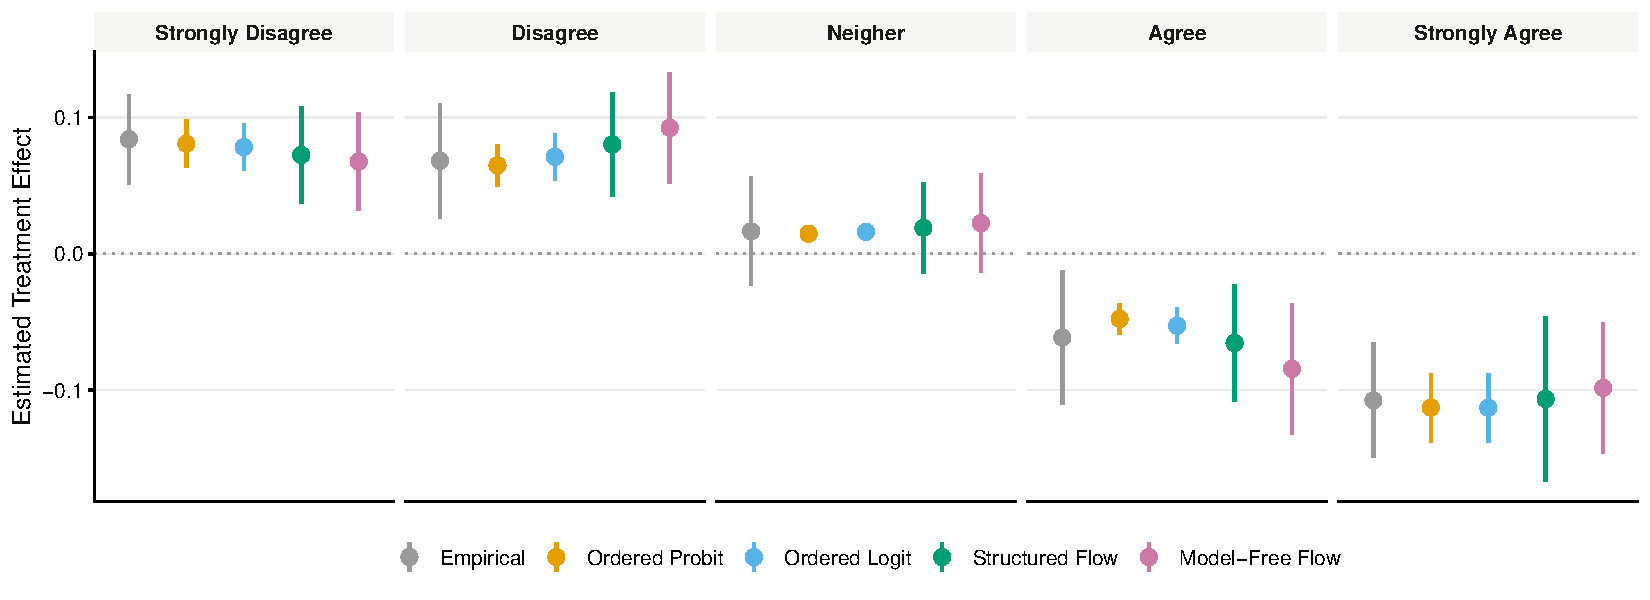
\includegraphics[width=0.95\textwidth]{../figures/fig_tomz_empirical.pdf}
  \end{center}
  \caption{Category Specific Effects on \citet{Tomz2020a}}\label{fig:tomz_empirical}
  \vspace{0.5em}
  \footnotesize
  \begin{flushleft}
    \textit{Note:} This figure reports the estimated category-specific treatment effects in replication of \citet{Tomz2020a}. Points denote category specific effect estimates and error bars indicate Bootstrapped 95\% Confidence Intervals.
  \end{flushleft}
\end{figure}

Figure~\ref{fig:tomz_empirical} compares the estimated category-specific treatment effects obtained from the empirical distribution estimator, ordered probit, ordered logit, and the two proposed flow-based estimators. Overall, the estimated treatment effects are remarkably consistent across estimation methods. All five approaches indicate that the treatment shifts respondents away from the highest levels of support for military intervention and toward lower response categories, with only modest differences in the estimated magnitudes. The structured flow estimator closely tracks the estimates produced by the classical ordered response models, while the model-free specification yields slightly greater uncertainty but no substantial change in the qualitative pattern of results.

This application illustrates an important point. Flexible estimation is not intended to replace conventional ordered response models regardless of context. Rather, it provides a robustness check against restrictive modeling assumptions. In this case, the substantive conclusions appear largely insensitive to the assumed latent error distribution, suggesting that the conventional ordered response models provide an adequate approximation for the observed data. The proposed estimator therefore reproduces the existing substantive findings while demonstrating that they are robust to substantially weaker distributional assumptions.

\subsection{\citet{Mattingly2025a}: Authoritarian Propaganda and Public Opinion}
\label{subsec:mattingly}

I next apply the flexible estimation framework to the survey experiment conducted by \citet{Mattingly2025a}, which examines the persuasive power of authoritarian state media on foreign public opinion. In this study, respondents were exposed to Chinese state propaganda and subsequently asked to report their relative preference for the United States versus the Chinese political system on a six-category ordinal scale, ranging from \emph{Strongly Prefer the US} (Category 1) to \emph{Strongly Prefer China} (Category 6). Standard empirical practice in this literature relies on ordered probit and logit models to estimate these persuasive treatment effects. 

\begin{figure}[ht]
  \begin{center}
  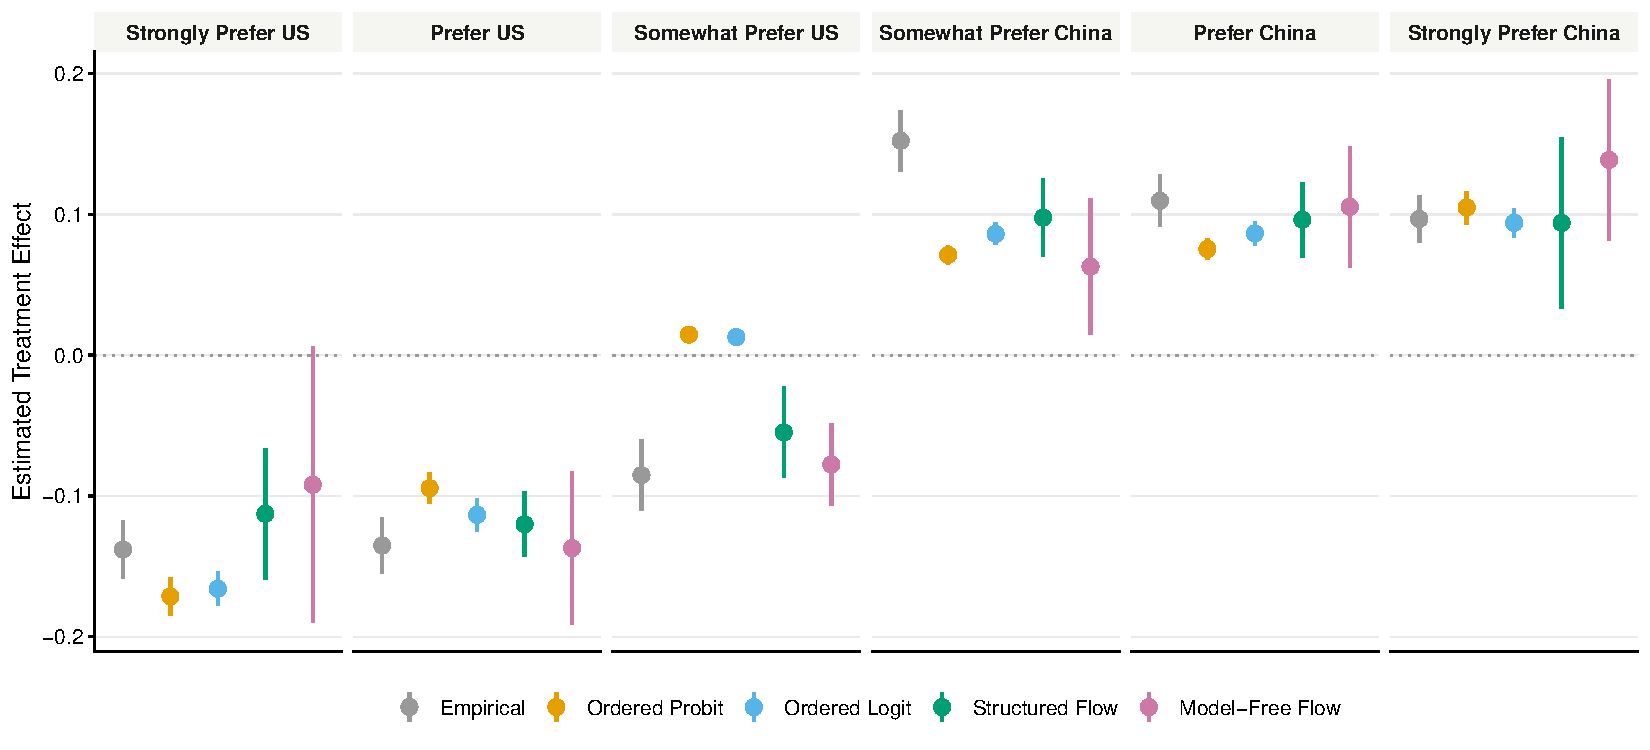
\includegraphics[width=0.95\textwidth]{../figures/fig_mattingly_empirical.pdf}
  \end{center}
  \caption{Category-Specific Effects in \citet{Mattingly2025a}}\label{fig:mattingly_empirical}
  \vspace{0.5em}
  \footnotesize
  \begin{flushleft}
    \textit{Note:} This figure reports the estimated category-specific treatment effects in the replication of \citet{Mattingly2025a}. Points denote category-specific average marginal effects, and error bars indicate bootstrapped 95\% confidence intervals.
  \end{flushleft}
\end{figure}

As shown in Figure~\ref{fig:mattingly_empirical}, all five estimators robustly agree on the broad direction of the treatment effect: the propaganda successfully shifts public opinion away from the US and toward China. Reassuringly, the overall qualitative pattern is stable across specifications, suggesting that the primary experimental finding is not a fragile artifact of a single statistical model. 

However, relaxing the rigid parametric constraints reveals a subtle but substantively interesting refinement in the estimated locus of persuasion. Standard parametric ordered models, by assuming a parallel shift of a fixed symmetric latent distribution, imply a relatively uniform movement of probability mass across the entire scale. Consequently, the ordered probit estimates a substantial 17 percentage point drop in the extreme \emph{Strongly Prefer US} category, but a near-zero effect on the moderate \emph{Somewhat Prefer US} category. 

By contrast, the flexible flow-based estimators suggest a more nuanced pattern of persuasion where treatment response may be heterogeneous across the distribution. While the confidence intervals are wide and overlap across estimators, the point estimates from the structured flow suggest a more moderate shift. The estimated drop in the extreme \emph{Strongly Prefer US} category is somewhat smaller (11 percentage points), while a notable 5 percentage point decrease is detected in the moderate \emph{Somewhat Prefer US} category. Additionally, the positive mass gained on the right side of the scale is concentrated slightly more heavily in the moderate \emph{Somewhat Prefer China} category under the flow estimators. 

While these differences do not overturn the original study's core finding that propaganda is persuasive, they suggest that conventional parametric models may slightly smooth over fine-grained variations in how soft supporters versus entrenched partisans respond to treatment. Substantively, the flexible model's estimates are consistent with a pattern where persuasion is concentrated among moderate leaners and soft opponents, while entrenched partisans are somewhat more resistant to the treatment.

Finally, this application provides an empirical illustration of the bias-variance tradeoff discussed in Section~\ref{sec:estimation}. While both the structured and model-free flows point toward the same pattern of moderate persuasion, the fully nonparametric model-free flow exhibits significantly larger uncertainty at the tails (e.g., in the \emph{Strongly Prefer China} category). The structured flow, by retaining the linear index to pool information across covariates, achieves much tighter confidence intervals. This supports our recommendation that the structured flow serves as a highly practical middle ground for analyzing moderate-sized survey experiments, offering distributional flexibility without sacrificing statistical precision.

\section{Conclusion}
\label{sec:conclusion}

Ordinal outcomes are among the most common outcome measures in political science, yet they present distinctive challenges for causal inference because the observed response categories reveal only the ordering of an underlying latent attitude. This paper revisited the classical identification result that latent treatment effects are identified only up to location and scale and argued that probability-based causal quantities defined on the observed ordinal responses provide a natural target for empirical analysis. Building on this perspective, I developed a flexible likelihood-based framework that estimates the conditional ordinal response distribution while relaxing the restrictive distributional assumptions imposed by conventional ordered response models.

The proposed framework retains the familiar latent-variable representation underlying ordered logit and ordered probit while replacing the fixed latent error distribution with a conditional normalizing flow. This construction preserves exact likelihood-based inference and accommodates both structured latent-index models and fully flexible conditional response distributions within a common estimation procedure. Rather than treating flexibility as an end in itself, the framework allows researchers to relax only those assumptions that are most difficult to justify while preserving the interpretability and statistical efficiency of classical ordinal response models.

The simulation study and empirical applications illustrate the practical consequences of this approach. When the assumptions underlying ordered response models are approximately correct, the proposed estimator performs comparably to conventional methods. When the latent response distribution departs from these assumptions, however, flexible estimation substantially improves recovery of both the conditional ordinal response distribution and the resulting distributional causal effects. The empirical applications further demonstrate that the sensitivity of substantive conclusions to distributional assumptions varies across studies. In some settings, conventional ordered response models provide essentially the same conclusions as the proposed estimator. In others, relaxing the latent error distribution meaningfully changes where in the ordinal response distribution treatment effects are estimated to occur.

More broadly, this paper argues that the conditional ordinal response distribution, rather than any single latent coefficient, should be viewed as the primary statistical object for causal inference with ordinal outcomes. Once this distribution has been estimated, a wide range of scientifically meaningful causal summaries, including category-specific effects, cumulative treatment effects, and other distributional functionals, follow naturally through standardization. This perspective separates the statistical problem of estimating the response distribution from the substantive problem of selecting the causal quantity most appropriate for a particular research question.

Several extensions remain for future work. The framework developed here assumes a common reporting function across respondents, whereas heterogeneous reporting behavior and measurement error remain important challenges for many survey instruments. Extending the proposed approach to multiple-item ordinal outcomes, integrating it with doubly robust estimation for observational studies, and developing formal specification diagnostics for parametric ordinal response models represent promising directions for future research.

As ordinal outcomes continue to play a central role in political science, the goal need not be to replace familiar ordered response models, but to extend them. Flexible likelihood-based estimation offers a practical way to preserve the strengths of classical ordinal models while reducing their dependence on restrictive distributional assumptions, thereby providing more robust causal inference when the underlying response process is uncertain.


\bibliographystyle{apsr}
\bibliography{/Users/chanhyuk/Documents/MyLibrary}

\end{document}
